\documentclass{elsarticle}

\usepackage[latin1]{inputenc}
\usepackage[T1]{fontenc}
\usepackage[english]{babel}
\usepackage{graphicx}
\usepackage{booktabs}
\usepackage{multirow}
\usepackage{color}
\definecolor{Red}{rgb}{.9,0,0}
%\usepackage{picins}


\newcommand{\fig}[4][htbp]{
  \begin{figure}[#1] {\centering\scalebox{#2}{\includegraphics{fig/#3}}\par}
    \caption{#4\label{#3}}
  \end{figure}
}

\newcommand{\multfigtwoh}[6][htbp]{
\begin{figure*}[#1]
  \centering
  \subfloat[]{\label{#3}\scalebox{#2}{\includegraphics{fig/#3}}}
  \subfloat[]{\label{#4}\scalebox{#2}{\includegraphics{fig/#4}}}
  \caption{#6}
  \label{#5}
\end{figure*}
}

\newcommand{\multfigtwov}[6][htbp]{
\begin{figure}[#1]
  \centering
  \subfloat[]{\label{#3}\scalebox{#2}{\includegraphics{fig/#3}}}\\
  \subfloat[]{\label{#4}\scalebox{#2}{\includegraphics{fig/#4}}}
  \caption{#6}
  \label{#5}
\end{figure}
}

\newcommand{\figR}[5][htbp]{
  \begin{figure}[#1]{\centering\scalebox{#2}{\includegraphics[angle=#5]{fig/#3}}\par}
    \caption{#4\label{#3}}
  \end{figure}
}

\newcommand{\figTC}[4][htbp]{
  \begin{figure*}[#1] {\centering\scalebox{#2}{\includegraphics{fig/#3}}\par}
    \caption{#4\label{#3}}
  \end{figure*}
}

\newcommand{\figEMPTY}[5][htbp]{
  \begin{figure}[#1]
    \fbox{\begin{minipage}{#2}\hfill\vspace{#3}\end{minipage}}
    \centering
     \label{#4}
    \caption{#5}
  \end{figure}
}

\newcommand{\tab}[3][htbp]{
  \begin{table}[#1]
    \footnotesize
    \centering
    \caption{#3}
    \include{tab/#2}
    \label{#2}
  \end{table}
}

\newcommand{\tabTC}[3][htbp]{
  \begin{table*}[#1]
    \footnotesize
    \centering
    \caption{#3}
    \include{tab/#2}
    \label{#2}
  \end{table*}
}

 %new commands


\journal{Microprocessors and Microsystems}

\begin{document}

\begin{frontmatter}

\title{Aspect-oriented RTL HW design using SystemC}

\author{T. R. M�ck\corref{cor1}\fnref{fn1}}
\ead{tiago@lisha.ufsc.br}
\author{A. A. Fr�hlich\fnref{fn1}}
\ead{guto@lisha.ufsc.br}
\address{Federal University of Santa Catarina, Florian�polis, Brazil}

\cortext[cor1]{Corresponding author}

\fntext[fn1]{Authors full address:\\
UFSC/CTC/LISHA\\
PO Box 476\\
88040-900 Florian�polis - SC - Brazil\\
Phone/Fax: +55 48 3721-9516 }

\begin{abstract}
With the increasing complexity of digital hardware designs, hardware description languages are
being pushed to higher levels of abstraction, thus allowing for the use of design artifacts which
were
previously exclusive to the software domain. In this paper we aim to contribute to this scenario by
proposing artifacts and guidelines for digital hardware design using object-oriented and
aspect-oriented programming concepts. Our methodology is based on features provided by SystemC, a
C++-based hardware description language, and leverages on its synthesizable subset in order to
produce designs suitable for circuit synthesis. Our experimental results show that our design
artifacts provide an increased level of flexibility and reusability while increasing the final
circuit size by only $2\%$
\end{abstract}

\begin{keyword}
aspect-oriented programming \sep digital hardware design \sep hardware description languages \sep SystemC
\end{keyword}

\end{frontmatter}

\section{Introduction}
\label{INTRO}
The complexity of digital hardware design is increasing as the advances of the semiconductor
industry allow for the use of sophisticated computational resources in a wider range of
applications. This new deployment scenario is leading to a growing interest in high-level
methodologies for
digital hardware design. Solutions and methodologies that have been successfully deployed in the
scope of large-scale software systems, such as \textit{object-oriented programming}~(OOP), are being
introduced to hardware design as well. An example of a \textit{hardware description language}~(HDL)
which supports OOP is SystemC, a C++-based HDL~\cite{Panda:2001}.

HDLs are used to create descriptions of electronic circuits which can be used either for design
verification or for hardware synthesis. Differently from most software programming
languages, HDLs are intrinsically parallel and provide explicit means for describing timing.
VHDL~\cite{VHDL:2000} and Verilog~\cite{Verilog:2001} are the most widely used HDLs for 
\textit{register transfer level}~(RTL) design. In RTL, circuits are described in terms of the
operations between storage elements which are synchronized using clock signals. In this level, a
hardware design may be composed by several \emph{modules}, whose instances are interconnected to
build the system. However, in contrast to software programming languages, module communication
occurs through timed protocols and signals defined by the module input/output interface instead of
function calls.

The use of OOP-capable HDLs (e.g. SystemC) enables an increased level of flexibility and reusability
in hardware design. Object-oriented features, such as inheritance and polymorphism, allow the
stepwise refinement and generalization of hardware IPs in a way it is not possible with standard
HDLs. However, analogous to software, in hardware some system-wide cross-cutting
concerns still cannot be elegantly encapsulated. For example, in complex circuits, interconnection
of several entities is realized by introducing buses. A bus physically interacts with other
components (e.g. CPU, DMA ...), but it is difficult to use a module or an OOP class to encapsulate
the bus because its interface and arbitration method have to be implemented in every attached
component~\cite{Engel:2008}. Other examples of cross-cutting concerns in hardware design can be
found in parts of a system related to its overall functionality or the implementation of
non-functional properties (e.g. fault-tolerance and low-power mechanisms, hardware debugging through
scan chains, clock handling, ...)~\cite{Endoh:2011}. Even by using OOP in hardware, this scattered
code is hard to maintain and bugs may be easily introduced. This motivates the introduction of
\emph{aspect-oriented programming}~(AOP)~\cite{Kiczales:1997} techniques for hardware design. 

AOP is an elaboration over OOP to deal with crosscutting concerns. AOP proposes the encapsulation of
these concerns in special classes called \emph{aspects}. An aspect weaving semantic is then defined
to describe when and how aspects are applied to components. The aspect weaving is defined
in terms of \emph{pointcuts} and \emph{join points}. The latter defines which points of a program
can be affected by an aspect, while the former defines when and how aspects are inserted at the
join points. Some extensions to OOP languages have been proposed to support these concepts. For
example, AspectJ~\cite{Kiczales:2001} and AspectC++~\cite{Spinczyk:2002} extend Java and C++ with
full support for AOP features. They provide both new language constructs and an aspect weaving
tool that applies aspects to the base code before it is processed by the traditional compiling
chain.

As can be seen in the next section, several works have already shown that the introduction of the
aforementioned concepts to hardware design is expected to provide means for the encapsulation of
cross-cutting concerns and an increase in the overall design quality. However, previous works in
this topic have focused on high-level specification and AOP features are used mostly for code
instrumentation and verification~\cite{Kallel:2010,Liu:2010,Vachharajani:2004}. Research targeting
the use of AOP for the actual design of hardware functionalities have proposed language constructs
and features which are not supported by hardware synthesis
tools~\cite{Endoh:2011,FengLiu:2009,Jun:2009,Deharbe:2006}, thus lacking a more comprehensive
discussion about the physical overhead related to the use of AOP in hardware.

In order to contribute to this scenario, in this paper we describe a digital hardware design method
which leverages on SystemC features in order to enable the implementation of hardware components
using OOP and AOP concepts. We propose the use of a design strategy that yields
components in which its dependencies from the execution scenario are encapsulated as \emph{aspects}
and \emph{configurable features}. The proposed aspect weaving semantics are implemented using only
standard C++, hence eliminating the need of extra tools and compilers.
Additionally, such features are within the SystemC synthesizable subset~\cite{systemc_subset}, thus
yielding \emph{synthesizable components}. Our method is finally illustrated by the design and
implementation of case studies extracted from an industrial \textit{Private Automatic Branch
Exchange} (PABX) application.

In summary, this work has the following contributions:
\begin{itemize}
 \item It provides a comprehensive analysis of related work in the area of AOP applied to
hardware design.
 \item It describes an AOP-based method for designing synthesizable hardware components.
 \item It presents the design and implementation of real world case studies, which allowed us to
elucidate the tradeoffs of AOP applied to hardware.
\end{itemize}

The remaining of this paper is organized as follows: section \ref{RELATED_WORK} presents a
discussion about related work; sections \ref{PROPOSAL} and \ref{RESULTS} presents our design
methodology and its evaluation through case studies; and section \ref{CONCLUSION} closes the paper
with our conclusions.

\section{Related work}
\label{RELATED_WORK}

Several works have already addressed the use of AOP concepts for hardware design. \emph{Engel and
Spinczyk}~\cite{Engel:2008} discussed the nature of crosscutting concerns in VHDL-based hardware
designs and proposed a hypothetical AOP extension for VHDL. In \emph{Bainbridge-Smith and
Park}~\cite{Bainbridge-Smith:2005} the authors discussed how the separation of concerns may relate
to different levels of algorithmic abstraction. They have mentioned the development of ADH, a new
HDL based on AOP, but further details about ADH are not mentioned. \emph{Burapathana et
al.}~\cite{Burapathana:2005} proposed the use of AOP concepts to sequential logic design.
Nevertheless, they focused on very simple and low level examples like flip-flops and logic gates.

There are also several works which proposed the use of AOP concepts mostly for 
hardware verification. \emph{Kallel et al.}~\cite{Kallel:2010} proposed the use of SystemC and
AspectC++ to implement assertion checkers. The authors focused on the
verification of
\textit{transaction-level models}~(TLM)~\cite{Cai:2003} in which transaction state updates are used
as
pointcuts. They provide a framework in which the user's verification classes extend base aspect
classes that implement the pointcuts and the verification primitives. In \emph{Vachharajani et
al.}~\cite{Vachharajani:2004} the authors developed the \textit{Liberty Structural
Specification Language}~(LSS). In LSS each module can declare instances which emit certain
events at runtime. These events behave like pointcuts of AOP. Each time a certain state is reached
or a value is computed, the instance will emit the corresponding event and user-defined aspects will
perform statistics calculation and reporting. \emph{Liu et al.}~\cite{Liu:2010} also proposed
AOP-based instrumentation, but focusing on high-level power estimation. They have developed a
methodology based on SystemC in which AspectC++ is used to define special power-aware aspects. 
These aspects are used as configuration files to link power-aware libraries with SystemC models.

Other works provide AOP features not only for verification, but also for the actual
design of hardware. \emph{D\'{e}harbe and Medeiros}~\cite{Deharbe:2006} present and assess possible
applications of AOP in the context of integrated system design by using SystemC with AspectC++.
Differently from the works discussed previously, they showed how AOP can be used to encapsulate some
functional characteristics of hardware components. They modeled as aspects the replacement policy of
a cache, the data type of an FFT, and the communication protocol between modules. However, only
simulation results are shown and they do not compare the implementation of aspect-based components
against components with all the functionalities hand-coded. In a similar work, \emph{Liu et
al.}~\cite{FengLiu:2009} implemented a SystemC model for a 128-bit floating-point adder and
described the implementation of the same model using AOP techniques. But, synthesis results are not
provided and the two models are compared only in terms of functionality to show that the AOP design
works like the original SystemC-only design. ASystemC~\cite{Endoh:2011} also extends SystemC in a
similar fashion, but, instead of using AspectC++, authors developed their own aspect weaver.
The new aspect language was introduced through different case studies involving high-level
estimation of circuit size, feature-configurable products, and assertion-based verification.
However, the evaluation of ASystemC also does not compare hardware generated using traditional
methods with their proposal. AspectVHDL~\cite{Meier:2012}, on the other hand, defines an aspect
weaving approach that can yield synthesizable code. However, using VHDL as the base language limits
the potential for reusability since OOP features are not supported.

Other works in this area follow different approaches. The \emph{e} programming
language~\cite{Vax:2007} was designed for modeling and verification of electronic systems and some
of its mechanisms can be used to support AOP features. Apart from its OOP features, \emph{e} has
some constructs to define the execution order of overloaded methods in inherited classes, which can
be used to define pointcuts and implement aspects. Indeed, this can be used to implement the
behavior of hardware components, but \emph{e} is more focused in high-level specification and there
is not any tool support for synthesis. \emph{Jun et al.}~\cite{Jun:2009} analyzed the application of
\textit{Aspectual Feature Module} ~(AFM)~\cite{Apel:2008} to HDLs. They have implemented a RISC
processor using SystemC and FeatureC++, and showed how AFM enables the incremental
development of hardware through the modularization of code fragments for the implementation of a
function. However, AOP is used only for encapsulation of verification code and the authors
do not provide synthesis results of the resulting code.

\section{Designing hardware components using scenario adapters and configurable features}
\label{PROPOSAL}

Previous works that explored the use of AOP in SystemC have relied on AspectC++. We have also based
our approach on methodologies which have been used in the
software domain. The \textit{Application-driven Embedded System
Design}~(ADESD)~\cite{Froehlich:2001} methodology elaborates on commonality and variability
analysis---the well-known domain decomposition strategy behind OOP---to add the concept of aspect
identification and separation at early stages of design. Throughout ADESD's domain engineering
process, the properties that transcend the scope of single abstractions are captured as
\emph{aspects}. Such aspects include mostly dependencies from the execution scenario and
non-functional properties. This enables components to be reused on different scenarios with the
application of proper \emph{aspects}. This aspect weaving is performed by constructs called
\emph{Scenario adapters}~\cite{Froehlich:2000}. 

Whether such guidelines can also be defined for designing hardware has not yet been investigated,
but nonetheless, SystemC enables the introduction of convenient C++ constructs to increase the
quality of hardware designs. This will be demonstrated in the next sections.

\subsection{Scenario adapters}
\label{PROPOSAL:SCENARIO_ADAPTER}

Scenario adapters were developed around the idea of components getting \emph{in} and \emph{out} of
an execution scenario, allowing actions to be executed at these points, therefore, a scenario must
define at least two different operations: \emph{enter} and \emph{leave}. These actions must take
place respectively before and after each of the component's operation in order to setup the
conditions required by the scenario. For example, in a compressed scenario, \emph{enter}
would be responsible to decompress the component's input data, while \emph{leave} would compress its
outputs. Figure \ref{fig_scenario_adapters_orig} shows the general structure of a scenario adapter.
The \emph{Scenario} class represents the execution scenario and incorporates, via aggregation, all
of the aspects which define its characteristics. Then, the adaptation of the component to the
scenario is performed by the \emph{Scenario Adapter} class using inheritance. Using classical AOP
terms, there is a \emph{join point} before and after each method of a component's public
interface, while the \emph{pointcuts} are defined by the scenario adapter.

\figSC[ht]{.6}{fig_scenario_adapters_orig}
{UML-based class diagram showing the general structure and behavior of a scenario adapter.}

In order to bring these ideas to hardware, the difference between hardware and software must be
considered. In the software domain, components are objects which communicate using method invocation
(considering an OOP-based approach), so the scenario adapters were originally developed to provide
means to efficiently wrap the method calls to an object. However, in a RTL design, components have
input and output signals  instead of a method or function interface. Notwithstanding, SystemC
provides features to separate the implementation of the communication interface from the behavior,
thus allowing us to use scenario adapters in way very similar to the one used in software.

\figSC[ht]{.6}{fig_systemc_module}
{SystemC description of a RTL component with a simple handshaking interface.}

Figure \ref{fig_systemc_module} shows a SystemC implementation of a component with the interface
separated from the behavior. SystemC defines hardware components by the specialization of the
\emph{sc\_module} class. Components communicate using special objects called \emph{channels}.
SystemC channels can be used to encapsulate complex communication protocols at register transfer or
higher levels of abstraction. However, these complex channels lie outside the SystemC synthesizable
subset, so we use only use \emph{sc\_in} and \emph{sc\_out} channels, which define simple RTL input
and output ports for components. The entry point for the component execution must be a method
defined as SystemC processes (\emph{Component::behavior}). The example below shows how this method
can be used for implementing the handshaking protocol (using channels \emph{op\_reg\_in} and
\emph{op\_req\_out}) and calling the method that implements the operation
(\emph{Component::operation}):

\footnotesize\begin{verbatim}
...
If (op_req_in) {
    op_rdy_out = 0;
    data_out.write(operation(data_in.read()));
    op_rdy_out = 1;
}
...
\end{verbatim}\normalsize

Apart from the signal-oriented interface, the scheduling of operations among clock cycles is another
important characteristic that differentiates a RTL SystemC implementation of a component from its
analogous software implementation in C++. SystemC allows for different styles to define timing. In
our components we use SystemC's clocked threads (\emph{SC\_CTHREAD}), in which all operations are
synchronized to a clock signal using \emph{wait()} statements. All operations defined between two
\emph{wait()} statements occur in the same clock cycle. By using \emph{wait()} statements one can 
describe the synchronization more clearly without the need of implementing explicit state
machines. Figure \ref{fig_sm_wait} shows this difference. It compares the synchronization of three
operations that must be executed in a loop in different clock cycles. The rightmost implementation
uses a \emph{SC\_METHOD} process, which provides an implementation style very similar to
VHDL/Verilog, while the leftmost shows the implementation using \emph{SC\_CTHREAD}.

\figSC[ht]{.6}{fig_sm_wait}
{A state machine implemented using \emph{SC\_CTHREAD} and \emph{SC\_METHOD}.}

By using these constructs, one can describe components susceptible for adaptation using scenario
adapters. However, other differences between software and RTL hardware design must be considered.
In software, the execution model is naturally sequential. A software OOP model may contain several
independent classes and still have a single and sequential execution flow, unless the designer
explicitly models parallelism. On the other side, in RTL hardware all modules runs in parallel,
and the operations inside the modules are also executed in parallel unless the designer explicitly
schedules them in different clock cycles. Taking this into account, we propose to define each aspect
as a single and independent hardware component. Figure \ref{fig_aspect_common} shows this
definition. 

\figSC[ht]{.6}{fig_aspect_common}
{Definition of aspects as a SystemC module.}

The aspects can use the same handshaking mechanisms described previously in order to make it easier
to synchronize their execution with the rest of the design. The class \emph{Aspect\_Common}
encapsulates this protocol as shown below: 

\vbox{
\footnotesize\begin{verbatim}
If (op_req_in) {
    op_rdy_out = 0;
    static_cast<Aspect*>(this)->trigger_behavior();
    op_rdy_out = 1;
}
else {
    op_rdy_out = 1;
    static_cast<Aspect*>(this)->idle_behavior();
}
\end{verbatim}\normalsize
}


\emph{Aspect\_Common} defines basic input/outputs signals and a SystemC process on which the aspect
behavior is going to execute. Each class defining an aspect inherits from \emph{Aspect\_Common} and
must implement at least two methods: \emph{Aspect::trigger\_behavior} defines the behavior
executed when an operation is triggered; and \emph{Aspect::idle\_behavior} defines the
behavior executed when the aspect is in an idle state. Notice that the aspect classes derive from
template instantiations of \emph{Aspect\_Common} using themselves as template parameters. This is
known as \textit{Curiously Recurring Template Pattern}~(CRTP)~\cite{Coplien:1995}, and we use it to
avoid the use of dynamic polymorphism, which is not supported for hardware synthesis. The final form
of the scenario adapter in hardware can be seen in Figure \ref{fig_scenario_and_adapter} (for
simplicity, some details already shown in Figures \ref{fig_systemc_module}, \ref{fig_sm_wait}, and
\ref{fig_aspect_common} are omitted). 

\figSC{.6}{fig_scenario_and_adapter}
{UML-based diagram of the final scenario adapter. Input/output signals are omitted for simplicity.}

The \emph{Scenario} class represents the execution scenario and incorporates, via aggregation, all
of the aspects which define its characteristics. It defines \emph{enter} and \emph{leave} methods to
encapsulate the implementation of the handshaking protocol which trigger the aspects. The piece of
code below shows how the scenario's \emph{enter} operation could be implemented:

{
\vbox{
\footnotesize\begin{verbatim}
while(op_rdy_0 &  ... & op_rdy_n)
    wait();

for all aspects {
    ...
    //set aspects inputs/outputs
    ...
    op_req_0 = 1;
    ...
    op_req_n = 1;
}
wait();
for all aspects {
    op_req_0 = 0;
    ...
    op_req_n = 0;
}
\end{verbatim}\normalsize
}

All aspects are triggered at the same time and executes in parallel, however, if required by a
component, each aspect can be executed sequentially in a specific order. This modification
can be performed by specializing the scenario for specific components. The piece of code below
illustrates this specialization. The first class definition is a default implementation of
\emph{Scenario}, while the remaining ones define specific implementations for different components.

\footnotesize\begin{verbatim}
template<class T> Scenario {...};

template<> Scenario<Component_0> {...};
...
template<> Scenario<Component_n> {...};
\end{verbatim}\normalsize

The adaptation of the component to the scenario is performed by the \emph{Scenario\_Adapter} class
via inheritance. The methods that implement the operations of the component are overridden in the
\emph{Scenario\_Adapter} class, which wraps the original methods with calls to the scenario's
\emph{enter} and \emph{leave}:

\footnotesize\begin{verbatim}
Scenario::enter();
Component::operation();
Scenario::leave();
\end{verbatim}\normalsize

Similarly to the implementation of the aspects, CRTP is used to avoid dynamic polymorphism. Calls
to operations inside \emph{Component::behavior} are performed using the same approach described for
the \emph{Aspect\_Common} class:

\footnotesize\begin{verbatim}
static_cast<Adapter*>(this)->operation();
\end{verbatim}\normalsize

\subsection{Configurable features}
\label{PROPOSAL:CONF_FEATURES}

Additionally to the aspect separation, several characteristics can be
identified by the designer as configurable features of the components. Such characteristics
represent fine variations within a component, which can be set in order to change slightly its
behavior or structure. 

Special template classes called \emph{Traits} are used to define which
characteristics of each component is activated. The code sample below shows the implementation of a
trait class and how it is referred inside an operation:

\footnotesize\begin{verbatim}
template <> struct Traits<Component>
{
    static const bool feature_1   = true;
    static const bool feature_2   = false;
    ...
    static const bool feature_n   = true;
};

...

void Component::operation(){
    ...
    if (Traits<Component>::feature_1) {
        ...
    }
    ...
}
\end{verbatim}\normalsize

Additional behavior is executed inside \emph{Component::operation} if
the feature \emph{feature\_1} is enabled. Since the condition in the \emph{if statement} can be
statically evaluated, the additional code is completely optimized away by the synthesis tool when
the condition is false.

Metaprogramming techniques~\cite{Czarnecki:2000} can be associated with the trait concept to also
modify the structure through inheritance. The example below shows how one can define the base class
of \emph{Component} as a configurable feature: 

\footnotesize\begin{verbatim}
public Component : 
    public sc_module,
    public 
    IF<Traits<Component>::feature_n,
        Base_Class_1,
        Base_Class_2>::Result 
{
   ...
};
\end{verbatim}\normalsize

The \emph{IF} metaprogram uses partial template specialization to return one of two specified types
based on a boolean value. Its implementation is shown below:

\footnotesize\begin{verbatim}
template<bool condition, typename Then, typename Else>
struct IF 
{ typedef Then Result; };

template<typename Then, typename Else>
struct IF<false, Then, Else>
{ typedef Else Result; };
\end{verbatim}\normalsize

Figure \ref{fig_config_features_uml} shows how this concept can be represented in a UML diagram.
The component definition indicates its features. In the case of conditional inheritance, both
possibilities are represented with a special notation at the relationship definition.

\figSC{.6}{fig_config_features_uml}
{UML representation for configurable features}

\subsection{ADESD and classic AOP}
Several previous works have already discussed aspect-oriented hardware design using SystemC and
proposed solutions based on classic AOP concepts using AspectC++.
Apparently,
AspectC++ provides more powerful mechanisms for aspect implementation then ADESD's scenario
adapters, especially when it comes to the definition of pointcuts. Scenario adapters were not 
designed to add behavior in specific points inside an operation. However, it is possible to
circumvent this limitation using other standard OOP and the proposed configurable features. For
example, in \emph{D\'{e}harbe and Medeiros}~\cite{Deharbe:2006} the replacement policy of a memory
cache and the data type of an FFT are encapsulated as aspects, while a straightforward alternative
would be to use inheritance and templates parameters.

It is also worth mentioning that the implementation of ADESD's mechanisms can be realized using only
standard C++/SystemC features. No extensions to the
language or an aspect weaving tool are required. Previous works focused on tools and mechanisms that
were deployed originally for software development (e.g. AspectC++), therefore limiting its use for
the generation of synthesizable hardware. For example, AspectC++ may introduces dynamic pointers
and objects that are outside the SystemC synthesizable subset\cite{systemc_subset}, thus allowing
the development of simulation-only models. Although simple aspects in AspectC++ lead to simple code
transformation, previous works showed no evidence that AspectC++ woven code can be synthesized. This
limits the evaluation of the physical overheads (e.g. silicon area and performance) associated to
AOP.

As can be seen in the following sections, the use of OOP, scenario adapters, and configurable
features yield synthesizable code, thus enabling the use of ADESD's mechanisms in all levels of the 
design process.


\section{Evaluation}
\label{RESULTS}
In this section we describe the experimental results of the evaluation of our approach. First, we
describe the components which are part of our case studies along with the scenario aspects that we
have identified. Then, we provide an evaluation of the designs, considering reusability and 
hardware synthesis results for both area and delay.

\subsection{Case studies}
\label{CASE_STUDY}
We have analyzed a PABX application from one of our
industry partners and designed some of its basic building blocks using the proposed design
artifacts. A PABX system is basically a commutation matrix that switches connections amongst
different input/output data channels. These channels are connected to phone lines (through an AD/DA
converter), tone generators, and tone detectors. The system also provides the transmission of voice
data through an Ethernet network to support \emph{voice over IP}~(VoIP) lines. The basic
components defined as case studies are described in more details below. All of them were designed
according to the guidelines described in section \ref{PROPOSAL}.

\textbf{Resource scheduler:} the PABX system is implemented over the \textit{Embedded Parallel
Operating System}(EPOS)~\cite{EPOS}. This case is a hardware implementation of the EPOS's
thread scheduler~\cite{Marcondes:2009:2}. A scheduler may perform operations both
synchronously (upon request by another component) or asynchronously (by preempting the execution of
another component). This complexity makes it a good case study. Furthermore, a hardware-implemented
scheduler reduces jitter and improves the support for real-time applications. Such characteristics
can provide a major impact in the PABX system, since each channel in the PABX central is handled in
software by a different thread.
    
\textbf{FIR filter:} \textit{finite impulse response}~(FIR) filters are some of the most frequently used and
well-known blocks in digital signal processing , thus offering a high reuse potential in a wide
range of application
domains. This motivated a careful and flexible design. The main feature of our filter is the support
to both complex and real arithmetic by using configurable feature, as shown in Figure
\ref{fig_fir_uml}. The interface and MAC core are implemented separately and inherited according
to the feature set.

\figSC{.6}{fig_fir_uml}
{FIR filter structure}
    
\textbf{DTMF detector:} a \textit{Dual-Tone Multi-Frequency}~(DTMF) detector~\cite{Xinyi:2010} is
responsible for detecting DTMF tones in the phone lines. It is a critical component in any PABX
system, thus was selected as a case study.


\subsection{Scenario aspects}
We have identified two different execution scenarios in our application domain: a \emph{debugged}
scenario and a \emph{compressed} scenario in which on-chip debugging and compression
of sampled data are required, respectively. Figure \ref{fig_all_aspects_uml_lite}
shows the aspects implemented for each scenario and their interface. The aspects inherit the basic
handshaking protocol from \emph{Aspect\_Common} (section \ref{PROPOSAL:SCENARIO_ADAPTER}) and
implement only their specific interface and operations. More details about the scenarios and its
aspects are given below.

\figSC{.5}{fig_all_aspects_uml_lite}
{The debug and compression scenarios implemented}

\textbf{Debugged scenario:} the upper part of Figure \ref{fig_all_aspects_uml_lite} shows the
aspects that can be part of a debugged scenario. Unlike previous works, which focused mostly on
simulation-time tracing and logging, we have focused on \emph{design for
testability}~\cite{Williams:1983} and implemented aspects for on-chip debugging using a JTAG scan
chain. The implemented aspects define the following debugging functionalities: \emph{Watched} causes
the state of a component to be dumped every time it is modified; \emph{Traced} causes every
operation execution to be signalized; and \emph{Profiled} counts the number of clock cycles used by
the component for each operation. The width of debugging signals within each aspect is defined as
template parameter in order to match the requirements of different components.

\textbf{Compressed scenario:} the lower part of Figure \ref{fig_all_aspects_uml_lite} shows the
aspects that can be part of a compressed scenario. These aspects provide means to compress digital
signals, thus reducing the number of bits required to either store or transmit them. The
\emph{Dynamic\_Range\_Compression} aspect provides operations to compress or expand the dynamic
range of a signal (i.e. the largest and smallest possible values of a signal) using a linear
transformation. The \emph{ADPCM\_Encoder/Decoder} aspects implement the same operations using an
\emph{adaptive differential pulse-code modulation}~(ADPCM) algorithm~\cite{adpcm} to convert
16-bit samples to 4-bit samples.

\subsection{Scenario adapters implementation}
Figure \ref{fig_case_study_all} shows how we have applied the aspects using scenario adapters (for
simplicity, details such as methods, ports, and some hierarchies are omitted). The highlighted
components are the scenario adapters, which applies the scenario aspects to the components,
yielding the following new cases: 

\textbf{Debugged scheduler:} the \emph{Scheduler\_Adapter} class implements the scenario
adapter for our scheduler. It inherits from the \emph{Scheduler} and \emph{Debugged\_Scenario}
classes, adding support for on-chip debugging. The \emph{Debugged\_Scenario} class incorporates the
aspects \emph{Profiled}, \emph{Traced}, and \emph{Watched}.

\textbf{Debugged FIR filter with dynamic range compression:} the \emph{FIR\_Adapter} class
adapts \emph{FIR} for both \emph{Debugged\_Scenario} and \emph{Compressed\_Scenario}. The
\emph{Compressed\_Scenario} class incorporates the aspects \emph{Dynamic\_Range\_Compression},
\emph{ADPCM\_Encoder}, and \emph{ADPCM\_Decoder}. This scenario exemplifies a situation when
scenario specialization is required, since both ADPCM and dynamic range compression may not be used
by the same component. In this case, the specialization of \emph{Compressed\_Scenario} for
\emph{FIR} incorporates only dynamic range compression. The final implementation compresses the
samples before the filter, and expands them afterwards, thus trading-off precision for resource
consumption.

\textbf{Debugged DTMF detector with ADPCM:} the \emph{DTMF\_Detector\_Adapter} follows the same
approach of \emph{FIR\_Adapter}. However, in this case study, the specialization of
\emph{Compressed\_Scenario} incorporates only the ADPCM aspects.


\figSC{.6}{fig_case_study_all}
{Overview of the aspect-oriented design. The highlighted components are the scenario adapters
implemented as case studies.}

\subsection{Experimental results}

We have evaluated the overhead introduced by our artifacts in our case studies by comparing the
aspect-oriented implementation described previously with an implementation in which the aspect's
behavior is \emph{hand-coded} in the core components. To evaluate the efficiency, we have
synthesized the designs to a physical circuit in a \textit{field-programmable gate
array}~(FPGA). To evaluate the reusability we have analyzed the number of lines of code in each case
study. 

\subsubsection{Reusability}

Table \ref{tab_results_code_total2} compares the number of lines of code of the scenario
adapters with the hand-coded versions of all case studies. Line \emph{Scenarios-adapted} shows the
number of lines for each design artifact in the scenario-adapted design. Line \emph{Hand-coded}
shows the number of lines when our approach is not used and the aspects are hand-coded in
the core components. The results show that the number of lines written is actually smaller in the
handed-coded designs. However, this only highlights the initial development overhead of providing a
modular implementation of aspects and scenarios. In the scenario-adapted implementations, about
$33\%$ of the written code is reused in at least two of our three case studies; while the
hand-coded implementation shares no common code. The code from the \emph{debugged scenario} and the
related aspects is reused across all case studies, while the code from the \emph{compressed
scenario} is partially reused since different specializations of this scenario are used in two
cases. 

\tabSC[ht]{tab_results_code_total2}
{Number of lines of code of all cases}

\subsubsection{Synthesis results}

We have synthesized our design to physical
circuits targeting an FPGA and analyzed their performance and size (area). Figure
\ref{fig_synth_flow} shows the synthesis flow. The SystemC designs are first converted to VHDL
descriptions using Celoxica's Agility 1.3. Then, Xilinx ISE 13.1 is used for both logic synthesis
and place-and-route (the process of fitting a circuit for a specific FPGA device). As our target
device we have chosen a Xilinx Virtex6 XC6VLX240T FPGA.

\figSC{.6}{fig_synth_flow}
{Design synthesis flow targeting FPGAs}

Table \ref{tab_results_fpga_sim} shows the number of \textit{slices} used (a configurable logic
element
in Xilinx's FPGA) and the \textit{longest path delay}~(LPD) of the three case studies. The LPD
represents the performance of the circuit, while the number of slices is used to evaluate the area.
The results show that the use of scenario adapters yields a very low overhead in terms of both
resource consumption and performance. The average area of the scenario-adapted components is about
$2\%$ higher than the hand-coded components. This small overhead comes basically from the additional
signal and registers required by the handshaking protocol that is used to trigger the aspects, which
is not required when everything is coded within a single SystemC module. The average difference in
performance is also small ($0.78\%$). Curiously, in the first case study, the scenario-adapted
design has a smaller LPD. This may be the result of some optimization algorithm applied in the
place-and-route backend.

\tabSC[ht]{tab_results_fpga_sim}
{FPGA synthesis results. Cases 1-3 refer to the scheduler, FIR, and DTMF detector, respectively.}


\section{Conclusion}
\label{CONCLUSION}

This paper has introduced an AOP-based method for designing hardware components using
SystemC. The components dependencies from different specific execution scenarios were successfully
encapsulated and further applied to
the core components through the use of scenario adapters and configurable features. By using the
proposed design strategy, on-chip debugging features were implemented as separated aspects and
fully reused throughout the case studies, thus showing the ease-of-use and versatility of
scenario-adapters to handle homogeneous crosscutting concerns.

The adaptation of components that require the addition of different behaviors in the same
execution scenario was also demonstrated. We have used partial template specialization to create a
compressed scenario that incorporates either dynamic range compression or ADPCM coding depending on
the component it is applied to. Although a full reusability  could not be achieved in this case, the
scenario specialization mechanism provides a straightforward and clear way to encapsulate
heterogeneous crosscutting concerns. 

In addition, we have also focused in the design of synthesizable hardware components, rather than
verification and simulation-only models. The experimental results showed that our design artifacts
can not only increase reusability but also be efficiently synthesized to physical hardware. The
scenario adapter structure and handshaking mechanisms for scenario activation increased the circuit
size by only $2\%$, while introducing a negligible overhead in the circuit performance.

\bibliographystyle{elsarticle-num}
\bibliography{paper}

%\section*{Author's biography}
%
%\parpic{
\includegraphics[width=1in,clip,keepaspectratio,natwidth=77,natheight=109]{fig_bio_tiago.png}}
%\noindent {\bf Tiago Rog�rio M�ck} received his B.Sc. in Computer Science from the Federal
%University of Santa Catarina, Brazil. He is currently a final year M.Sc. student in the Computer
%Science Department at the same university. His current research interests include computer 
%architecture and embedded systems.
%
%\vspace{12mm}
%
%\parpic{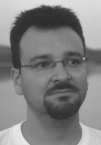
\includegraphics[width=1in,clip,keepaspectratio,natwidth=101,natheight=145]{fig_bio_guto.png}}
%\noindent {\bf Antonio Augusto Fr�hlich}
%received his Ph.D. in Computer Science from the Technical University of Berlin in 2001. He has been
%a professor in the Computer Science Department, Federal University of Santa Catarina, Brazil
%since 1995 and head of the Laboratory for Software and Hardware Integration since 2001. His current
%research interests include embedded systems and operating systems.

\end{document}
